\chapter{Hidden Markov models}
\label{sec_hmm}
In this chapter we consider probabilistic graphical models of the form shown in figure \ref{fig_linmod}. We assume that  $(X_0, X_1,\hdots)$ are each $n$ state discrete random variables and that $(Y_0, Y_1,\hdots)$ are each $m$ state discrete random variables. Models of this form are classically called hidden Markov models.
\begin{figure}[H] 
\centering
\begin{tikzpicture}

  % Define nodes
  \node[obs] (ya) {$Y_{0}$};
  \node[latent, above=of ya]  (xa) {$X_{0}$};
  \node[obs, right=of ya] (yb) {$Y_{1}$};
  \node[latent, above=of yb, right=of xa]  (xb) {$X_1$};
  
  % Connect the nodes
  \edge {xa} {ya};
  \edge {xa} {xb};
  \edge {xb} {yb};
  
\end{tikzpicture}
\caption{Graphical model used in this chapter.}
\label{fig_linmod}
\end{figure}
Intuitively, this model represents the situation where we are not sure about the state of the world but we can observe some facet of it. At each time step our state changes stochastically according to the transition function. A new observation is (stochastically) generated from our new state. Generally, we attempt to infer the state of the world given the observations. Clearly two new random variables $X_t, Y_t$ are created at each time step.

In this chapter we briefly describe Markov models because they link back to previous work done by the chemical engineering department at the University of Pretoria. We focus on hidden Markov models for the remainder of the chapter because the techniques we develop here generalise to linear latent dynamical systems which we discuss in chapter \ref{sec_inf_lin_mods}. 

\section{Markov models}
A first order Markov model (sometimes called a Markov chain) is shown in figure \ref{fig_markov_chain}. Using the chain rule for Bayesian networks (definition \ref{def_chain_rule_bayes}) we can immediately write down the joint probability distribution
\begin{equation}
P(X_{0:T}) = \Pi_{t=0}^T P(X_t|X_{t-1}) \text{ with } P(X_0|X_{-1}) = P(X_0).
\label{eq_markov_chain_joint}
\end{equation}  
\begin{figure}[H] 
\centering
\begin{tikzpicture}

  % Define nodes
  \node[latent]  (xa) {$X_{0}$};
  \node[latent, right=of xa]  (xb) {$X_{1}$};
  \node[latent, right=of xb]  (xc) {$\hdots$};
  \node[latent, right=of xc]  (xd) {$X_{T-1}$};
  \node[latent, right=of xd]  (xe) {$X_{T}$};
  % Connect the nodes
  \edge {xa} {xb};
  \edge {xb} {xc};
  \edge {xc} {xd};
  \edge {xd} {xe};
\end{tikzpicture}
\caption{First order markov chain.}
\label{fig_markov_chain}
\end{figure}
This model describes the forward propagation of a discrete random variable through time. It is interesting to study the marginal distribution of $P(X_T)$ as it evolves through time. By d-separation we know that $X_t \indep X_{0:t-2} | X_{t-1}$. Thus, we only have to marginalise out the previous time step to compute the required distribution 
\begin{equation}
P(X_T) = \sum_{x_{T-1}} P(X_T, x_{T-1}) = \sum_{x_{T-1}} P(x_{T-1})P(X_T|x_{T-1}).
\label{eq_markov_chain_marg}
\end{equation}
Since we know that the transition function is a row stochastic $n \times n$ matrix (the random variable has $n$ discrete states) we can write (\ref{eq_markov_chain_marg}) in vector notation 
\begin{equation}
P(X_t) = \mathbf{p}_t = \mathbf{A}\mathbf{p}_{t-1} = \mathbf{M}^{t-1}\mathbf{p}_1.
\label{eq_markov_chain_marg_vec}
\end{equation}
Note that $P(X_T)$ is a discrete random variable and can thus be expressed as a stochastic column vector i.e. $\sum_i P(x_t=i) = 1$. We have implicitly rewritten (\ref{eq_markov_chain_marg_vec}) in recursive format. Thus, we have a recursive expression for the marginal distribution of $X$. If, as $T \rightarrow \infty$, we have that $\mathbf{p}_{t \rightarrow \infty} = \mathbf{p}_{\infty}$ exists and is independent of $\mathbf{p}_0$ we call $\mathbf{p}_{\infty}$ the equilibrium distribution of the chain. 

We define the stationary distribution, in matrix notation, by \begin{equation}
\mathbf{p}_{\infty} = \mathbf{A}\mathbf{p}_{\infty}.
\label{eq_markov_chain_stationary}
\end{equation}
Recalling the definition of the eigenvalue problem we see that the stationary distribution is just the eigenvector corresponding to the unit eigenvalue of $\mathbf{A}$. While this model may seem simplistic it is the foundation of Google's PageRank algorithm \cite{google}.  Intuitively $\mathbf{p}_\infty$ represents the steady state probability distribution of the random variable $X$ as it is propagated through time by the transition function $A$. See the work in \cite{streicher} for an application specifically geared towards chemical engineering.

\section{Hidden Markov models}
Hidden Markov models extend Markov models by incorporating the observed random variables $(Y_0, Y_1,\hdots)$ as shown in figure \ref{fig_linmod}. At each time step it is now possible to observe the random variable $Y_t$ which gives more information about the state of $X_t$. We are still in the setting of discrete random variables. It is not necessary to restrict $(Y_0, Y_1,\hdots)$ to be discrete but we do so for the sake of simplicity here. In later chapters we will model both hybrid and purely continuous systems. 

In general a hidden Markov model is just a specific case of the general dynamic Bayesian network class of graphical models. As such we already know that to fully specify the model we only require a prior state distribution $P(X_0)$, the transition probability function $P(X_t|X_{t-1})$, the observation (or sometimes called the emission) probability function $P(Y_t|X_t)$ and the Bayesian network graphs of the initial time step and the next two time steps. We assume that the model's structure repeats at each time step and thus we only require the graph as shown in figure \ref{fig_linmod}.

We assume that the transition and observation probability functions are stationary. Consequently they may be represented by the row stochastic square matrices $P(x_t=i|x_{t-1}=j) = A$ and $P(y_t=i|x_t=j) = B$. Intuitively this means that the probability of state $x_{t-1}=j$ going to state $x_{t} = i$ is $A_{ij}$. Similarly, $B_{ij}$ is the probability of observing $y_t=i$ if the underlying state is $x_t=j$.

For the purposes of this dissertation we will always assume that the model parameters are known. In section \ref{sec_dbns_lit} the four primary inference techniques were briefly mentioned. We now derive recursive expressions for each inference technique for discrete models of the form shown in figure \ref{fig_linmod}. The tools and techniques we develop here will be useful in the following chapters. 

\subsection{Filtering}
The goal of filtering is to find $P(X_t|y_{0:t})$: the distribution of the current state given all the past and current observations. The corresponding graphical model is shown in figure \ref{fig_linmod_filter_hmm}.
\begin{figure}[H] 
\centering
\begin{tikzpicture}

  % Define nodes
  \node[obs] (ya) {$Y_{0}$};
  \node[latent, above=of ya]  (xa) {$X_{0}$};
  \node[obs, right=of ya] (yb) {$\cdots$};
  \node[latent, above=of yb, right=of xa]  (xb) {$\cdots$};
  \node[obs, right=of yb] (yc) {$Y_{t-1}$};
  \node[latent, above=of yc, right=of xb]  (xc) {$X_{t-1}$};  
  \node[obs, right=of yc] (yd) {$Y_t$};
  \node[latent, above=of yd, right=of xc]  (xd) {$X_t$};  
  
  % Connect the nodes
  \edge {xa} {ya};
  \edge {xa} {xb};
  \edge {xb} {yb};
  \edge {xb} {xc};
  \edge {xc} {yc};
  \edge {xc} {xd};
  \edge {xd} {yd};

\end{tikzpicture}
\caption{Filtering graphical model.}
\label{fig_linmod_filter_hmm}
\end{figure}
We start the derivation by noting that $X_{t-1}$ d-separates $X_t$ from $X_{0:t-2}$. Thus $X_{t-1}$ contains all the hidden state information of the system up to and including $t-1$. This is not surprising since we have assumed a first order Markov system. This is why we only marginalise over the reduced state joint $P(X_t, X_{t-1}|y_{0:t})$ in
\begin{equation}
\begin{aligned}
P(X_t| y_{0:t-1}) &= \sum_{x_{t-1}} P(X_t, x_{t-1}| y_{0:t-1})\\
&= \sum_{x_{t-1}} P(x_{t-1}|y_{0:t-1})P(X_t|y_{0:t-1}, x_{t-1})\\  
& = \sum_{x_{t-1}} P(x_{t-1}|y_{0:t-1})P(X_t|x_{t-1}).
\end{aligned}
\label{eq_forward_no_recur}
\end{equation}
The expansion followed from the chain rule of Bayesian networks (definition \ref{def_chain_rule_bayes}) and the cancellation followed from the conditional independence assumption of the transition function. Next we define $\alpha(X_t) \equiv P(X_t | y_{0:t})$; then
\begin{equation}
\begin{aligned}
\alpha(X_t) &= \frac{P(y_t|X_t, y_{0:t-1})P(X_t|y_{0:t-1})}{P(y_t|y_{0:t-1})} \\
& = \frac{P(y_t|X_t)P(X_t|y_{0:t-1})}{P(y_t|y_{0:t-1})} \\
& = \frac{P(y_t|X_t) \sum_{x_{t-1}} P(x_{t-1}|y_{0:t-1})P(X_t|x_{t-1})}{P(y_t|y_{0:t-1})} \\
& = \frac{P(y_t|X_t) \sum_{x_{t-1}} \alpha(x_{t-1})P(X_t|x_{t-1})}{P(y_t|y_{0:t-1})} \\
\end{aligned}
\label{eq_forward_recur}
\end{equation}
follows from (\ref{eq_forward_no_recur}) and by application of Bayes' theorem (theorem \ref{thrm_bayes}). It is not actually necessary to calculate $p(y_t|y_{0:t-1})$ as it is only a normalisation constant. We thus have a recursion relation for the filtered posterior distribution $X_t$ with initial condition $\alpha(X_1) = P(X_1, y_1) = P(X_1)P(y_1|X_1)$ by
\begin{equation}
\alpha(X_t) \propto P(y_t|X_t) \sum_{x_{t-1}} \alpha(x_{t-1})P(X_t|x_{t-1}).
\label{eq_forward_approx}
\end{equation}
One often uses logarithms to perform the filter calculations as machine precision errors become a problem for large $t$ due to the multiplication of small fractions. The recursive filtering algorithm we derived is often called the forwards algorithm in literature \cite{barber}.

\subsection{Smoothing}
The goal of smoothing is to find $P(X_t|y_{0:T})$ for $t\leq T$: the distribution of the state at $t$ given all the past and future observations to $T$. The smoothing algorithm we study here is called the parallel smoothing algorithm. The recursion expression we derive is often called the backwards algorithm in literature \cite{murphy1}. The graphical model corresponding to this situation is shown in figure \ref{fig_linmod_smooth_hmm}.
\begin{figure}[H] 
\centering
\begin{tikzpicture}

  % Define nodes
  \node[obs] (ya) {$Y_{0}$};
  \node[latent, above=of ya]  (xa) {$X_{0}$};
  \node[obs, right=of ya] (yb) {$\cdots$};
  \node[latent, above=of yb, right=of xa]  (xb) {$\cdots$};
  \node[obs, right=of yb] (yc) {$Y_{t}$};
  \node[latent, above=of yc, right=of xb]  (xc) {$X_{t}$};  
  \node[obs, right=of yc] (yd) {$\cdots$};
  \node[latent, above=of yd, right=of xc]  (xd) {$\cdots$};  
  \node[obs, right=of yd] (ye) {$Y_T$};
  \node[latent, above=of ye, right=of xd]  (xe) {$X_T$};  
  
  % Connect the nodes
  \edge {xa} {ya};
  \edge {xa} {xb};
  \edge {xb} {yb};
  \edge {xb} {xc};
  \edge {xc} {yc};
  \edge {xc} {xd};
  \edge {xd} {yd};
  \edge {xd} {xe};
  \edge {xe} {ye};

\end{tikzpicture}
\caption{Smoothing graphical model.}
\label{fig_linmod_smooth_hmm}
\end{figure}
We start by splitting the joint $P(X_t, y_{0:T}) = P(X_t, y_{0:t})P(y_{t+1:T}|X_t,y_{0:t})$ by the chain rule and using d-separation to reduce it further $P(X_t, y_{0:T}) = P(X_t, y_{0:t})P(y_{t+1:T}|X_t)$. Effectively the last step implies that future observations are independent of past observations given the current state. We defined $\beta(X_t)\equiv P(y_{t+1:T}|X_t)$ and continue
\begin{equation}
\begin{aligned}
P(y_{t:T}|X_{t-1}) &= \sum_{x_t} P(y_t, y_{t+1:T}, x_t|X_{t-1}) \\
&= \sum_{x_t} P(y_{t+1:T}, x_t | X_{t-1})P(y_t| y_{t+1:T}, x_t, X_{t-1}) \\
&= \sum_{x_t} P(y_{t+1:T}, x_t | X_{t-1})P(y_t| x_t) \\
&= \sum_{x_t} P(x_t | X_{t-1})P(y_{t+1:T}| x_t,X_{t-1})P(y_t| x_t) \\
&= \sum_{x_t} P(x_t | X_{t-1})P(y_{t+1:T}| x_t)P(y_t| x_t).
\end{aligned}
\label{eq_backwards_no_recur}
\end{equation}
We have made judicious use of the implied independence assertions (via d-separation) of figure~\ref{fig_linmod}. Making use of the definition of $\beta$ we have
\begin{equation}
\begin{aligned}
&\beta(X_{t-1}) = \sum_{x_t} P(x_t | X_{t-1})\beta(x_t)P(y_t| x_t) \text{ for } 1 \leq t \leq T \\
&\text{with } \beta(X_T) = 1.
\end{aligned}
\label{eq_backwards_recur}
\end{equation}
The recursion initial condition $\beta(X_T) = 1$ stems from Bayes' theorem (theorem \ref{thrm_bayes}) and the definition of $\alpha$ as illustrated by
\begin{equation}
\begin{aligned}
P(X_T|y_{0:T}) &= \frac{P(X_T, y_{0:T})}{P(y_{0:T})} \\
&= \alpha(X_T) \beta(X_T)\\
&= P(X_T| y_{0:T}) \beta(X_T)\\
&\implies \beta(X_T) = 1.
\end{aligned}
\label{eq_backwards_recur_initial}
\end{equation}
Note that $\beta$ is not a probability function. The smoothed posterior is given by applying Bayes' theorem
\begin{equation}
P(X_t|y_{0:T}) = \frac{\alpha(X_t)\beta(X_t)}{\sum_{x_t}\alpha(x_t)\beta(x_t)}.
\label{eq_smooth}
\end{equation}
Together the $\alpha - \beta$ recursions are called the forwards-backwards algorithm and find extensive use in general purpose exact inference of dynamic Bayesian networks \cite{murphy1}.

Numerical issues may also become problematic due to the multiplication of small positive numbers. In practice it is often necessary to work in the log space to attenuate these problems~\cite{barber}. 

\subsection{Viterbi decoding}
The goal of Viterbi decoding is to find $x_{0:T}^* = \underset{x_{0:T}}{\text{arg max }} P(x_{0:T}|y_{0:T})$: finding the most likely sequence of states which best describe the observations by  attempting to find the sequence $x_{0:T}$ such that the joint probability function $P(x_{0:T}, y_{0:T})$ is maximised. This is equivalent to finding $ \underset{x_{0:T}}{\text{arg max }} P(x_{0:T}|y_{0:T})$ because, if one uses the chain rule on the joint, the observations will just be a constant factor. The graphical model used here is similar to that of figure \ref{fig_linmod_smooth_hmm}.

Intuitively we first attempt to find the maximum of the joint and then determine which sequence of states led to this maximal joint. By using the chain rule for Bayesian networks we can rewrite the joint maximisation problem as
\begin{equation}
\begin{aligned}
\underset{x_{0:T}}{\text{max }} P(x_{0:T}, y_{0:T}) &= \underset{x_{0:T}}{\text{max }} \Pi_{t=1}^T P(y_t|x_t) P(x_t|x_{t-1})\\
&= \left(\underset{x_{0:T-1}}{\text{max }} \Pi_{t=1}^{T-1} P(y_t|x_t) P(x_t|x_{t-1}) \right) \underset{x_{T}}{\text{max }} P(y_T|x_T) P(x_T|x_{T-1}).
\end{aligned}
\label{eq_viterbi_joint}
\end{equation}
Defining $\mu(X_{t-1}) \equiv \underset{x_{t}}{\text{max }} P(y_t|x_t) P(x_t|x_{t-1})$ we can rewrite (\ref{eq_viterbi_joint}) as \begin{equation}
\underset{x_{0:T}}{\text{max }} P(x_{0:T}, y_{0:T}) =\underset{x_{0:T-1}}{\text{max }} \Pi_{t=1}^{T-1} P(y_t|x_t) P(x_t|x_{t-1}) \mu(x_{T-1}).
\label{eq_viterbi_max_factor_mu}
\end{equation}
Thus we have a recursive expression,
\begin{equation}
\begin{aligned}
&\mu(x_{t-1}) = \underset{x_{t}}{\text{max }} P(y_t|x_t) P(x_t|x_{t-1}) \mu(x_t) \text{ for } 2 \leq t \leq T \\
&\text{with } \mu(x_T) = 1, 
\end{aligned}
\label{eq_viterbi_recur}
\end{equation}
to find the value of the joint under the most likely sequence of states given the observations.

The recursive expression in (\ref{eq_viterbi_recur}) implies that the effect of maximising over the previous time step can be compressed into a message (a function) of the current time step. Effectively we pass theses messages backward in time to find the maximum joint in terms of $x_0$. We then find the state which maximises this joint and pass this message forward.  Continuing in this way we have
\begin{equation}
\begin{aligned}
x_1^* &= \underset{x_{1}}{\text{arg max }}P(y_1|x_1)P(x_1)\mu(x_1) \\
x_2^* &= \underset{x_{2}}{\text{arg max }}P(y_2|x_2)P(x_2|x_1^*)\mu(x_2) \\
&~~\vdots \\
x_t^* &= \underset{x_{t}}{\text{arg max }}P(y_t|x_t)P(x_t|x_{t-1}^*)\mu(x_t).
\end{aligned}
\label{eq_viterbi_recur_forward}
\end{equation}
This algorithm is called the Viterbi algorithm. It is computationally efficient since the optimisations occur only on a single variable. Readers familiar with dynamic programming will recognise that we have effectively performed a variant of dynamic programming in the preceding derivation.

\subsection{Prediction}
The goal of prediction is to find $P(X_{t+1}|y_{0:t})$ and $P(Y_{t+1}|y_{0:t})$: the predicted hidden and observed state given all the previous observations. The one step ahead prediction expression for both the states and observations is derived here. The graphical model corresponding to the state prediction is shown in figure \ref{fig_linmod_pred_hmm}. 
\begin{figure}[H] 
\centering
\begin{tikzpicture}

  % Define nodes
  \node[obs] (ya) {$Y_{0}$};
  \node[latent, above=of ya]  (xa) {$X_{0}$};
  \node[obs, right=of ya] (yb) {$\cdots$};
  \node[latent, above=of yb, right=of xa]  (xb) {$\cdots$};
  \node[obs, right=of yb] (yc) {$Y_{t}$};
  \node[latent, above=of yc, right=of xb]  (xc) {$X_{t}$};  
  \node[latent, above=of yd, right=of xc]  (xd) {$X_{t+1}$};  
  
  % Connect the nodes
  \edge {xa} {ya};
  \edge {xa} {xb};
  \edge {xb} {yb};
  \edge {xb} {xc};
  \edge {xc} {yc};
  \edge {xc} {xd};
  
\end{tikzpicture}
\caption{State prediction graphical model.}
\label{fig_linmod_pred_hmm}
\end{figure}
We again start by noticing that given all the observations  up to time $t$ the current state d-separates  all previous states. Thus, to infer information about the next state we only need to marginalise out the current state $X_t$. Furthermore, the next state d-separates the next observation from all the previous states. Thus, to infer information about the next observation we additionally only need to marginalise out $X_{t+1}$.

We start with predicting the next state distribution. We have applied the chain rule, the independence assertions and used the definition of $\alpha$ to write
\begin{equation}
\begin{aligned}
P(X_{t+1}|y_{0:t}) &= \sum_{x_t} P(X_{t+1}, x_t|y_{0:t}) \\
&= \sum_{x_t} P(x_t|y_{0:t})P(X_{t+1}|x_t, y_{0:t}) \\
&= \sum_{x_t} P(x_t|y_{0:t})P(X_{t+1}|x_t) \\
&= \sum_{x_t} \alpha(x_t)P(X_{t+1}|x_t).
\end{aligned}
\label{eq_prediction_state}
\end{equation}
Clearly the state prediction uses the filtered state estimate and projects that forward using the transition function. Next we derive the observation prediction. Again we apply the chain rule, use the independence assertions and use the definition of $\alpha$ to write
\begin{equation}
\begin{aligned}
P(Y_{t+1}|y_{0:t}) &= \sum_{x_t, x_{t+1}} P(x_{t+1}, x_t, Y_{t+1}|y_{0:t})\\
&= \sum_{x_t, x_{t+1}} P(x_t|y_{0:t})P(x_{t+1}, Y_{t+1}|y_{0:t}, x_t) \\
&= \sum_{x_t, x_{t+1}} P(x_t|y_{0:t})P(x_{t+1}|y_{0:t}, x_t)P(Y_{t+1}|y_{0:t}, x_t, x_{t+1}) \\
&= \sum_{x_t, x_{t+1}} P(x_t|y_{0:t})P(x_{t+1}|x_t)P(Y_{t+1}|x_{t+1}) \\
&= \sum_{x_t, x_{t+1}} \alpha(x_t)P(x_{t+1}|x_t)P(Y_{t+1}|x_{t+1}).
\end{aligned}
\label{eq_prediction_observation}
\end{equation}
Clearly the observation prediction is just an extension of the state prediction. We effectively just predict the next state and use the observation function to predict the observation distribution.

It is pleasing that the prediction expressions are closely related to each other and effectively only depend on the filtered state estimate and the transition or observation functions. This realisation hold for more general problems and will become important when we consider controlling the system. More on this later.

\section{Burglar localisation problem}
While the focus of this dissertation is not on hidden Markov model type problems it is nevertheless instructive to consider a simple example to build some intuition about inference of random variables. Thus, it is desirable to conduct a numerical experiment using the previously derived inference techniques. The type of problem we consider here is a localisation problem. This type of problem (and its extensions) has many applications in robotics and object tracking.

The problem is taken from chapter 23 in Barber's book \textit{Bayesian Reasoning and Machine Learning} \cite{barber}. Briefly, it is necessary to infer the location of a burglar in your house given observations (noises) you perceive from an adjoining room. You discretise the room the burglar is in into $n^2$ blocks. The room is then the discrete random variable $X$. You observe two distinct types of noises: creaks and bumps. From the knowledge of your house you know which blocks are likely to creak and which are likely to bump if the burglar is on that block i.e. if the random variable $X$ is in a specific state. This is shown in figure \ref{fig_burlgar_observations}: a dark block indicates it is likely to emit a noise with probility 0.9 and a light block will emit a noise with probability 0.01 if the burglar is on that block. The noises are independent of each other.
\begin{figure}[H] 
\centering
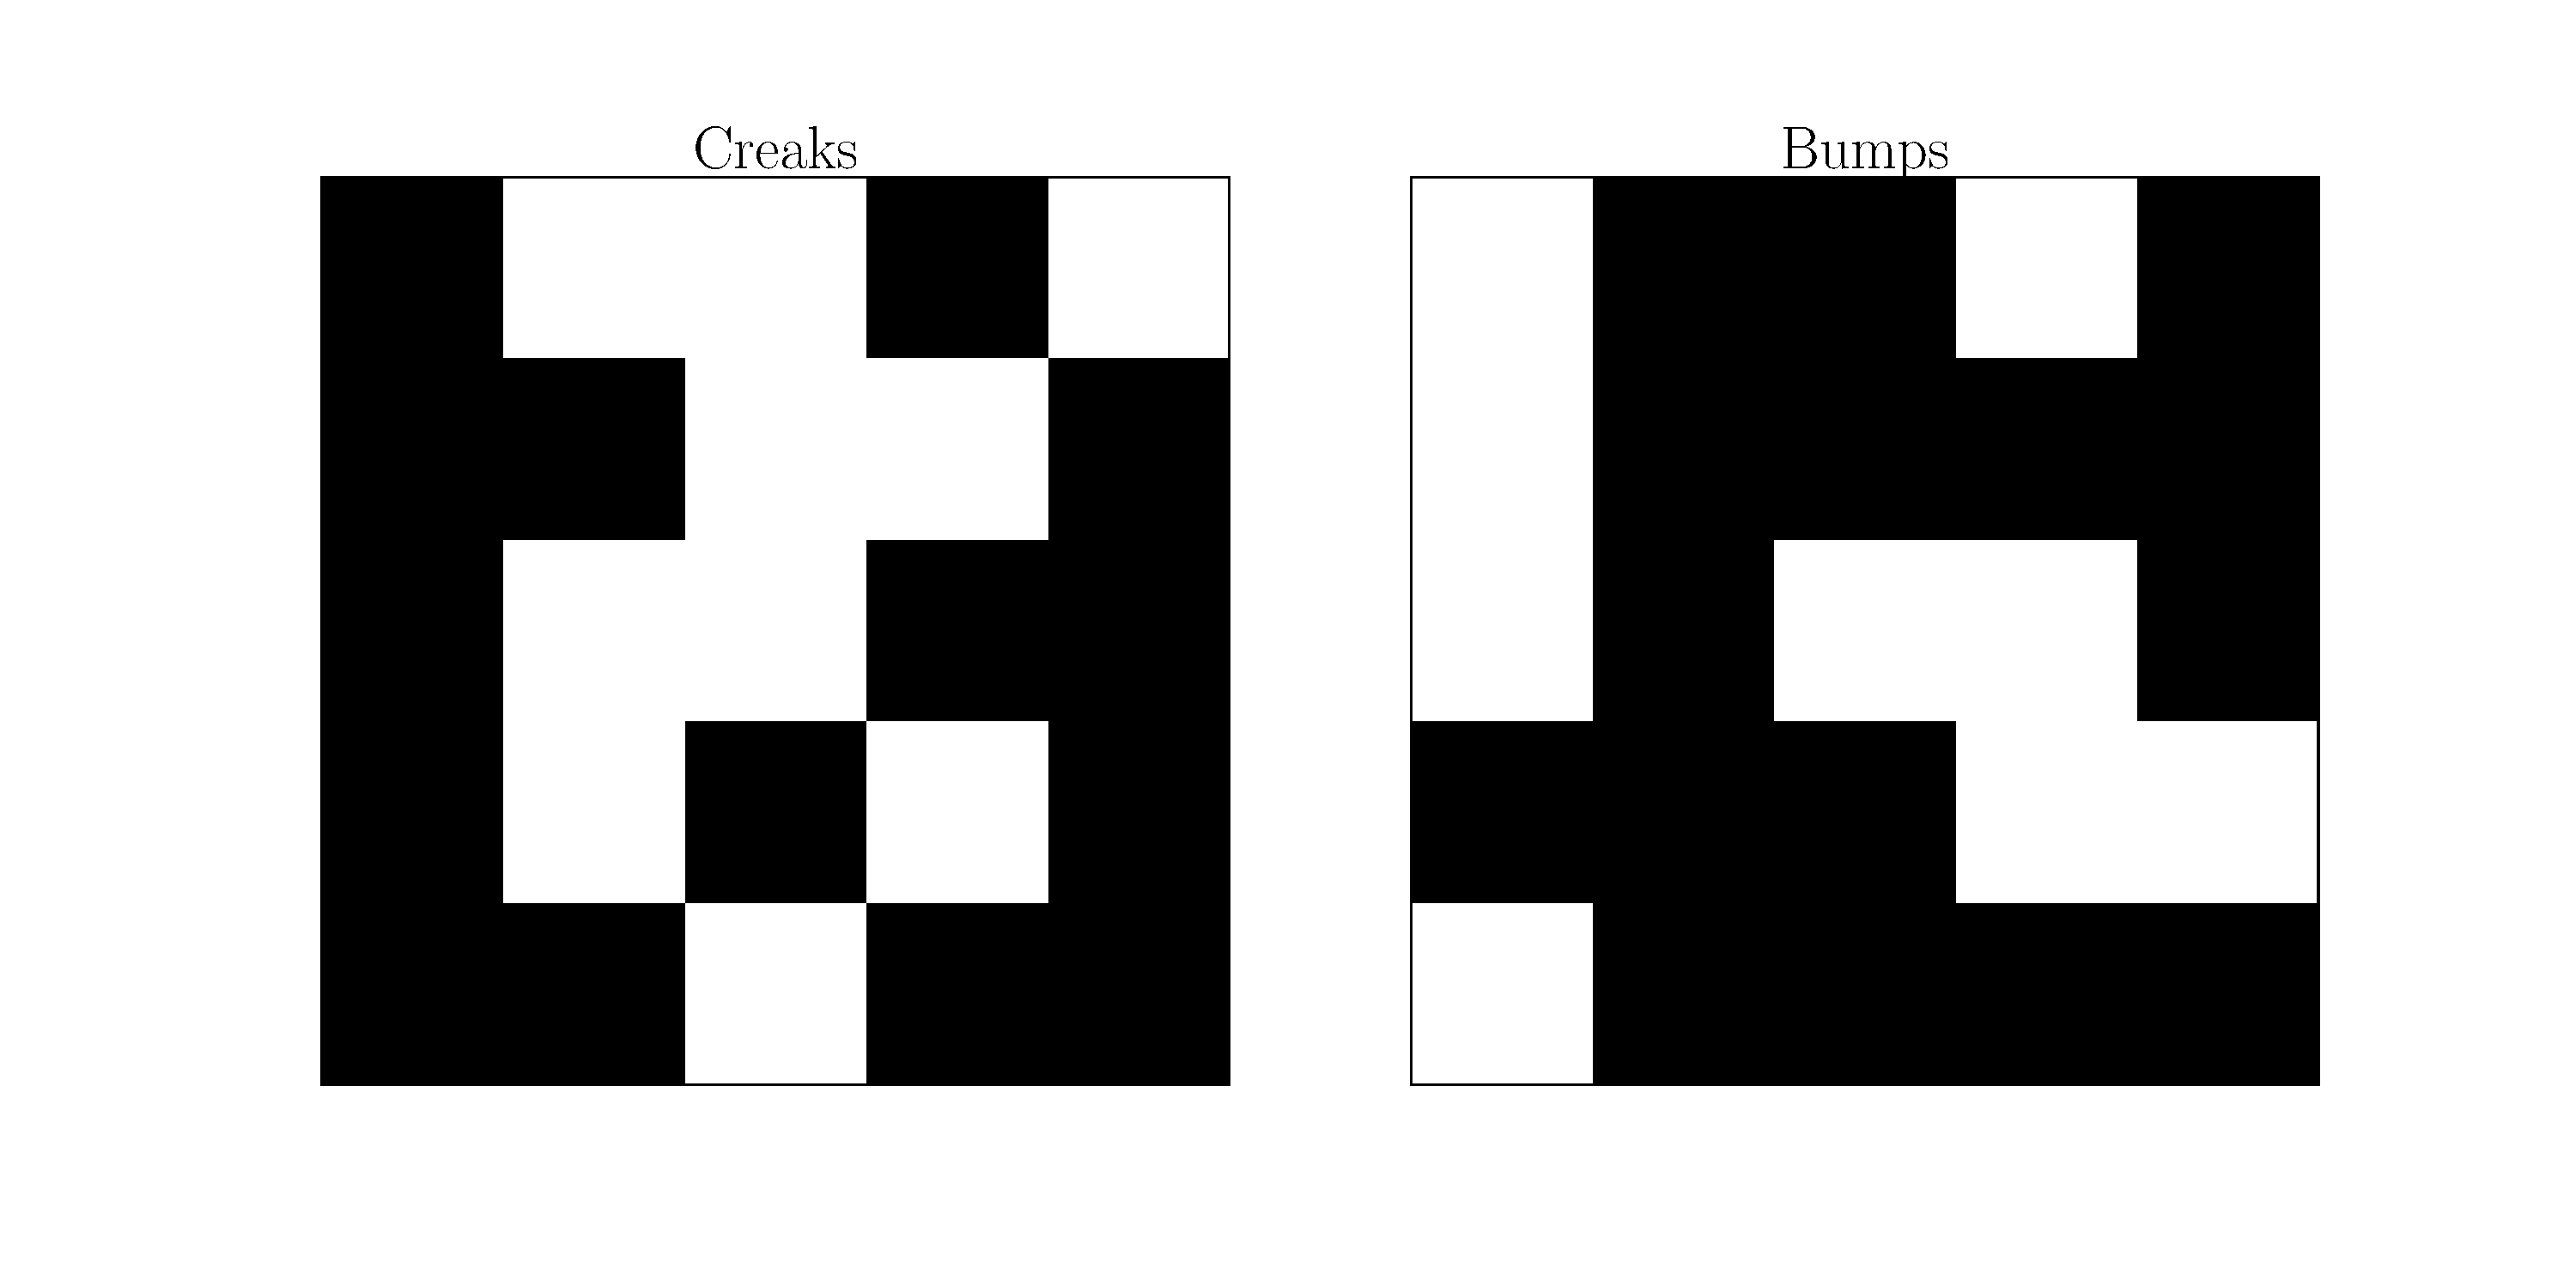
\includegraphics[scale=0.25]{burglar_observations.pdf}
\caption{Burglar problem observations.}
\label{fig_burlgar_observations}
\end{figure}
The burglar moves up, down, left and right with equal probability where appropriate. See Barber for more details on the example. It is necessary to perform inference to determine the path of the burglar both in real time and with the benefit of hindsight. Applying the inference techniques we developed earlier results in figure \ref{fig_burglar_inference}. 
\begin{figure}[H] 
\centering
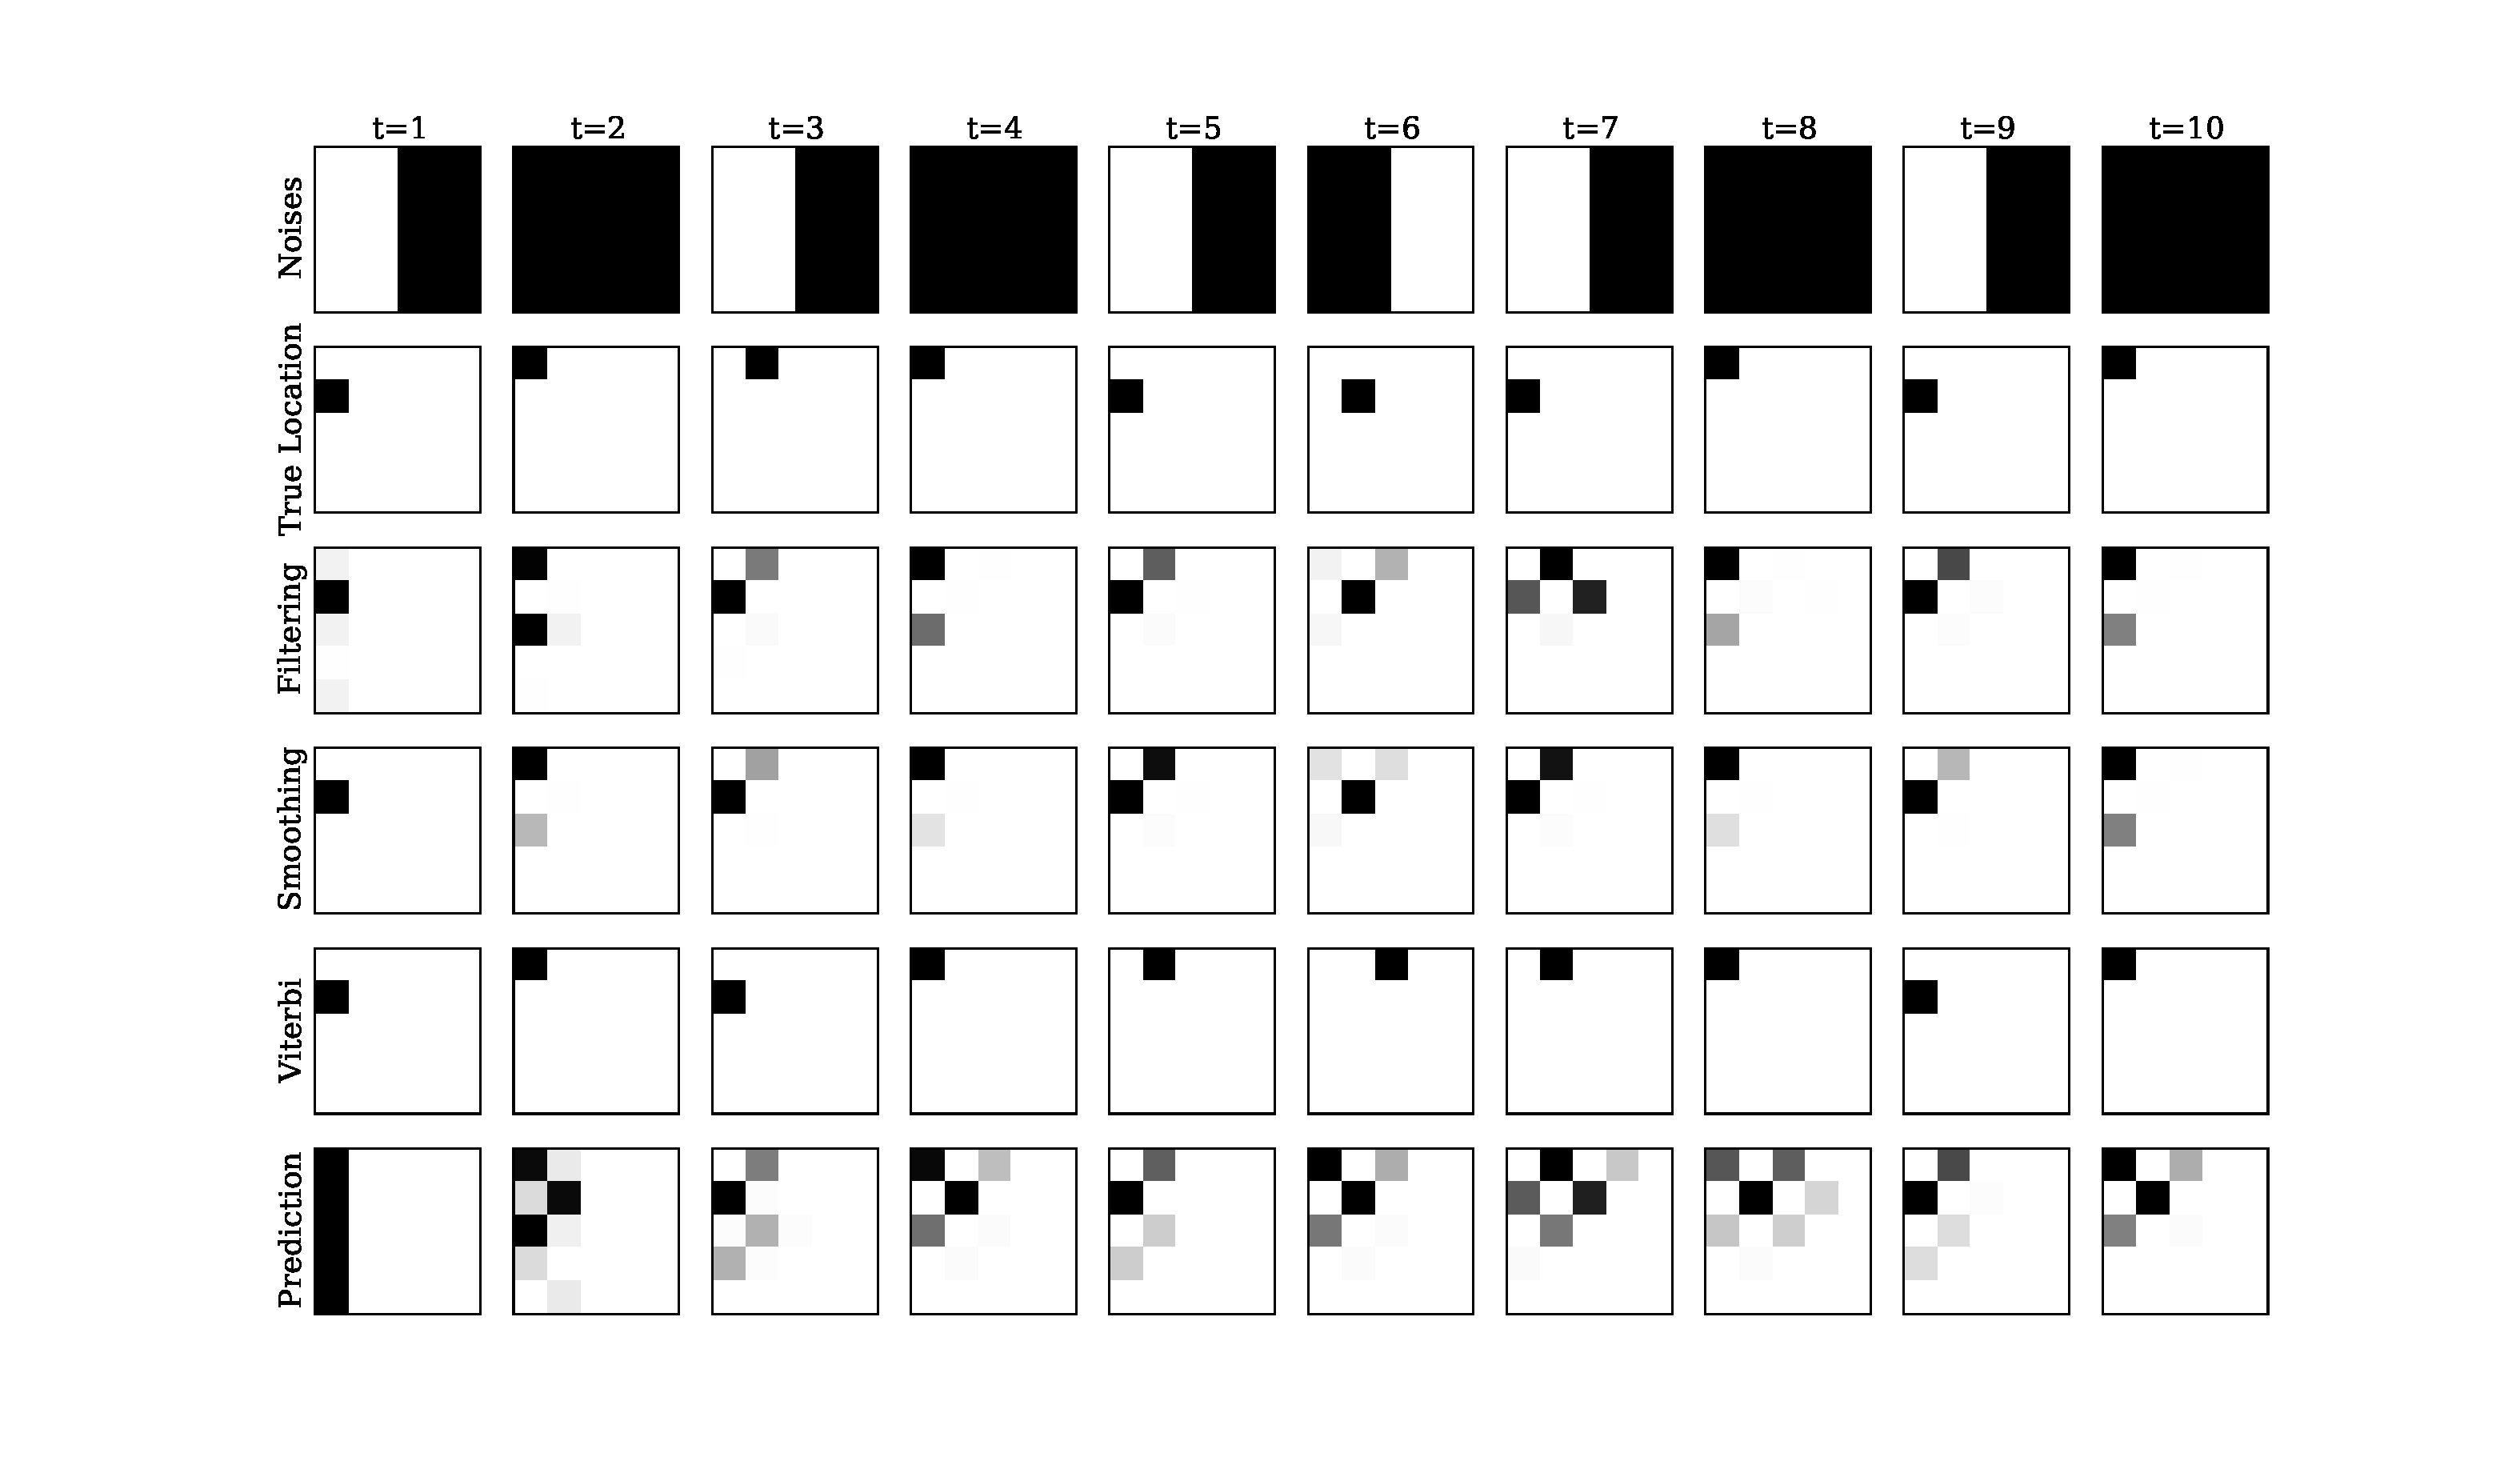
\includegraphics[scale=0.3]{burglar_inference.pdf}
\caption{Burglar problem: filter, smoothing, Viterbi decoding and prediction.}
\label{fig_burglar_inference}
\end{figure}
In this context filtering means we estimate the location of the burglar given all the past observations at the current time step. This inference can be done on-line. Smoothing means we attempt to estimate his position with hindsight given all the observations starting from the first time step and moving forwards. In Viterbi decoding we attempt to estimate the most likely path path of the burglar. Finally the prediction algorithm is self-explanatory.

It is interesting to note that smoothed posterior converges to the filtered posterior near the end of the time window. Reflecting on the expression for smoothing this is not surprising since at $t=T$ the smoothing component of the forwards-backwards algorithm is unity. Therefore we see that the smoothed state estimate converges to the filtered state estimate as $t$ approaches $T$.

It is also interesting to note that the prediction algorithm is very much dependent on the quality of the transition function. The four block pattern readily apparent in the prediction distribution originates from the transition function (the burglar is equally likely to move in any direction). This strongly implies that the closer the transition function is to reality the better our predictions will be.

Finally, it is important to understand the benefit of using this approach as opposed to the exhaustive ``if this then that" approach. Firstly, the latter approach scales exponentially with the number of variables because one would need to fully consider all the possibilities to infer any sort of belief. Secondly, the former approach has an associated probability distribution: the certainty of our inferred belief is automatically quantified e.g. the darker the blocks the more sure we are about our inference. Thus, the techniques we developed make room for uncertainty about the correctness of the answer.

Hidden Markov models are very powerful and have found many uses e.g. speech recognition, object tracking and bio-informatics \cite{barber}. Many extensions of the basic model (see figure \ref{fig_linmod}) exist which are much more expressive. However, we are interested in modelling and reasoning about continuous random variables. For such applications the hidden Markov model, due to the discrete assumption, is inappropriate. Fortunately, the techniques investigated in this chapter carry over to the continuous case as we will see in chapter \ref{sec_inf_lin_mods}.  
